%
% mexican.tex -- Mexikaner-Hut Wavelet
%
% (c) 2019 Prof Dr Andreas Müller, Hochschule Rapperswil
%
\documentclass[tikz]{standalone}
\usepackage{amsmath}
\usepackage{times}
\usepackage{txfonts}
\usepackage{pgfplots}
\usepackage{csvsimple}
\usetikzlibrary{arrows,intersections,math}
\begin{document}
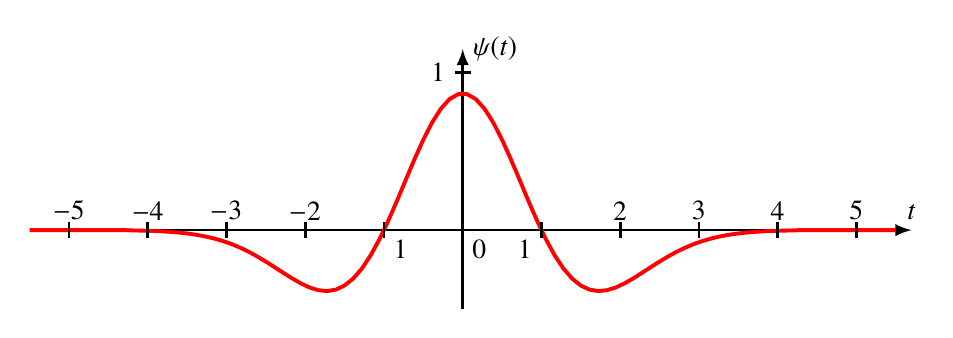
\begin{tikzpicture}[>=latex]

\def\s{2*0.867325}

\draw[->,line width=1pt] (-5.5,0)--(5.7,0) coordinate[label={$t$}];
\draw[->,line width=1pt] (0,-1)--(0,2.3) coordinate[label={right:$\psi(t)$}];

\draw[line width=1.4pt,color=red] plot[domain=-5.5:5.5,samples=100]
	({\x},{\s*(1-\x*\x)*exp(-\x*\x/2)});

\foreach \x in {-5,...,5}{
	\draw[line width=1pt] ({\x},-0.1)--({\x},0.1);
}
\draw[line width=1pt] (-0.1,2)--(0.1,2);
\node at (-0.1,2) [left] {$1$};

\node at (1,0) [below left] {$1$};
\node at (-1,0) [below right] {$1$};
\node at (0,0) [below right] {$0$};
\foreach \x in {2,...,5}{
	\node at ({\x},0) [above] {$\x$};
	\node at ({-\x},0) [above] {$-\x$};
}

\end{tikzpicture}
\end{document}

